
\chapter{Planning}
\label{sec:org2610146}
\section{Requirements}
\label{sec:org945b9f4}
\subsection{Safety and Security}
\label{sec:org34def69}
\begin{itemize}
\item Access control with different levels of security for different purposes e.g. medical cabinet, and 24/7 building access.
\item Surveillance of the public spaces
\item Smoke detection
\item Window and door status listed in the central hub
\item Safe deposit of monitoring feeds
\end{itemize}
\subsection{24/7 real-time Health Monitoring facilities}
\label{sec:orge43b7b8}
\begin{itemize}
\item Monitoring of inhabitants without breaking the laws of privacy
\item Heart rate
\item Location tracking
\item Blood pressure
\item Emergency button
\end{itemize}
\subsection{Engineering services}
\label{sec:org3b95898}
\begin{itemize}
\item Central hub that lists the status of the building infrastructure 
\item A silent alarm to the personal if a critical device is failing
\end{itemize}
\subsection{Energy and water consumption}
\label{sec:orgd85891f}
\begin{itemize}
\item Monitoring of water and energy consumption
\item Central heating control
\end{itemize}
\subsection{Cleanliness and outbuilding services}
\label{sec:orga2926ad}
\begin{itemize}
\item Tracking of cleaning services
\item An easy way to report contaminations
\end{itemize}
\subsection{Residents satisfaction}
\label{sec:orgd7a0521}
\begin{itemize}
\item A pleasant living temperature all year round that each individual can set in his own room
\item Optional registration for health services like heart rate and location tracking
\item Info board for events
\end{itemize}

\section{Specifications}
\label{sec:org1cd7898}

\subsection{Safety and Security}
\label{sec:orgdf376cf}
\begin{enumerate}
\item Access control with different levels of security for different purposes e.g. medical cabinet, and 24/7 building access.
\label{sec:orgfd41c27}
\begin{itemize}
\item Authorization / Authentication (REST, OAuth2.0)
\item Roles
\end{itemize}
\begin{center}
\begin{tabular}{lllllll}
 & Admin & Medical Staff & Technical Staff & residents & cleaning staff & manager\\
\hline
survaillance of public spaces & x &  & x &  &  & \\
state of windows and doors & x & x & x &  &  & \\
smoke alarms & x & x & x &  &  & \\
heart rate / blood pressure & x & x &  &  &  & \\
location tracking & x & x &  &  &  & \\
managing information for info board & x & x &  &  &  & \\
technical state of all devices & x &  & x &  &  & \\
update cleaning status of a room & x &  &  &  & x & \\
confirming cleaning status of a room & x &  &  &  &  & x\\
reading reports & x & x & x &  &  & x\\
access the info board & x & x & x & x &  & \\
\end{tabular}
\end{center}



\item Surveillance of the public spaces
\label{sec:org073d37f}
\begin{itemize}
\item video cameras for (hardware purchase and installation)
\begin{itemize}
\item parking lot
\item entrances
\item lunch area
\item chill room
\item communical area
\item elevators
\end{itemize}
\item archive backup file system
\begin{itemize}
\item NAS with redundance (RAID 2)
\item Backup also with (RAID 2)
\item label the files with location and timestamp for searching later
\end{itemize}
\end{itemize}
\item Smoke detection
\label{sec:orgd44eac6}
\begin{itemize}
\item In every room or corridor
\item Smoke detectors with network capabilities
\item Tracking the alarms with within the system (location and time)
\item Dashboard should be able visualize alarms origin
\end{itemize}

\item Window and door status listed in the central hub
\label{sec:org4d440ca}
\begin{itemize}
\item Buy wireless detectors/ sensors for doors and windows
\item Create interface for sensors to communicate with the central system
\item Dashboard should visualize the state of the doors and windows
\end{itemize}
\item Safe deposit of monitoring feeds
\label{sec:orgc8e70b4}
\begin{itemize}
\item Central system needs a database for persitent data storage
\item Redudant backup system
\end{itemize}
\end{enumerate}

\subsection{24/7 real-time Health Monitoring facilities}
\label{sec:orgb3edcb5}
\begin{enumerate}
\item Monitoring of inhabitants without breaking the laws of privacy
\label{sec:orgd852888}
\begin{itemize}
\item Buy motion detectors ( + installation)
\item Create interface for detectors to communicate with the backend
\item Dashboard should visualize the data of the motion detectors for each room
\end{itemize}

\item Health Monitoring
\label{sec:org97d117c}
\begin{itemize}
\item Heart rate  monitoring with smart wrist bands
\begin{itemize}
\item wrist band communicate with the backend
\item not mandatory for every resident - resident can decide for their own (or doctor orders it)
\item realtime monitoring via frontend for each resident who has a wrist band by their location (GPS)
\item implement alarm logic, when monitored health data shows critical state
\item alarm when dementia patient is near entrance (though RFID)
\end{itemize}

\item Emergency button
\begin{itemize}
\item purchase emergency buttons that can communicate with a central hub or backend
\item installation and create interface for communication with backend
\item log the frequency of the usage of each button (location / time) and store it in the database
\item provide access to the logs by the frontend and implement searching and filtering features
\end{itemize}
\end{itemize}
\end{enumerate}

\subsection{Engineering services}
\label{sec:org6af4132}
\begin{enumerate}
\item Central hub that lists the status of the building infrastructure
\label{sec:orgeccf6fd}
\begin{itemize}
\item A silent alarm to the personal if a critical device is failing
\item technical staff should be able to access the state of devices that are out of order
\begin{itemize}
\item sensors
\item lights
\item elevators
\item heating
\end{itemize}
\end{itemize}
\item ticket system for manual issue managment and tracking their state
\label{sec:orge41382f}
\begin{itemize}
\item technical staff and medical staff can manage the issues (add, update, delete)
\item design and implement a GUI for the staff that allows them to manage the issues
\end{itemize}
\end{enumerate}

\subsection{Energy and water consumption}
\label{sec:orged4964c}
\begin{enumerate}
\item Monitoring of water and energy consumption
\label{sec:org2364917}
\begin{itemize}
\item Design and implement a GUI for the technical staff to monitor the consumption
\item Buy smart power meters and water meters that can communicate with the backend
\item Log and aggragate the data in the database
\item Implement filtering and searching features for the stored data
\end{itemize}
\item Central heating control
\label{sec:org2012d7b}
\begin{itemize}
\item Residents can control the room temperature
\item Purchase heating controls that can communicate with the backend (installation and integration into  the system)
\item Purchase temperature sensors that can communicate with the backend (installation and integration into  the system)
\item Dashboard should visualize the temperature and heating settings of each room
\end{itemize}
\end{enumerate}
\subsection{Cleanliness and outbuilding services}
\label{sec:org14b7883}
\begin{enumerate}
\item Tracking of cleaning services
\label{sec:org20c4fcd}
\begin{itemize}
\item design and implement a GUI for the medical staff to save the date and room for which the cleaning service was done
\item implement backend and database for storing the data
\end{itemize}
\item An easy way to report contaminations
\label{sec:orgc4fa354}
\begin{itemize}
\item design an GUI for HMI-panels that provide an easy way to report contaminations
\begin{itemize}
\item should be placed in all public rooms
\item the GUI should have buttons for different kind of urgent problems
\begin{itemize}
\item cleaning service
\item emergency
\end{itemize}
\end{itemize}
\item design and implement a GUI for the medical staff to report contaminations
\item implement backend and database for storing the data
\end{itemize}
\end{enumerate}
\subsection{Residents satisfaction}
\label{sec:org903f351}
\begin{enumerate}
\item CORE
\label{sec:orgaf1de29}
\begin{itemize}
\item automatic feedback generation based on input of manager (food quality, room
temperature, cleanliness of rooms, (maybe) staff kindness)
\end{itemize}
\item Optional registration for health services like heart rate and location tracking
\label{sec:org0528d08}
\begin{itemize}
\item design and implement a GUI for the medical staff for storing which person was given a wrist band
\item implement backend and database for storing the data
\end{itemize}
\item Info board for events
\label{sec:orgcba1be4}
\begin{itemize}
\item Purchase flat screen (installation and integration in the system)
\item Web frontend that is also accessable on mobile devices
\item implement backend and database for storing the data
\end{itemize}
\end{enumerate}


\subsection{Technical Specification}
\label{sec:org896d172}
\begin{itemize}
\item Settings Page
\item timer for checking for critical states of
\begin{itemize}
\item windows, door states
\item heart rate
\end{itemize}
\item Database for data persitents
\item RFID instead of GPS for location tracking
\item generate templates for reports
\item mobile app for android tablets (for medical staff and cleaning staff, manager)
\end{itemize}




\section{Implementation}
\label{sec:orgaa7b811}

\section{Basic Concept}
Based on the requirements and specifications presented in the previous chapters, the architecture was designed as shown in the following figure \ref{architecure}:
\begin{figure}[H]
	\centering
	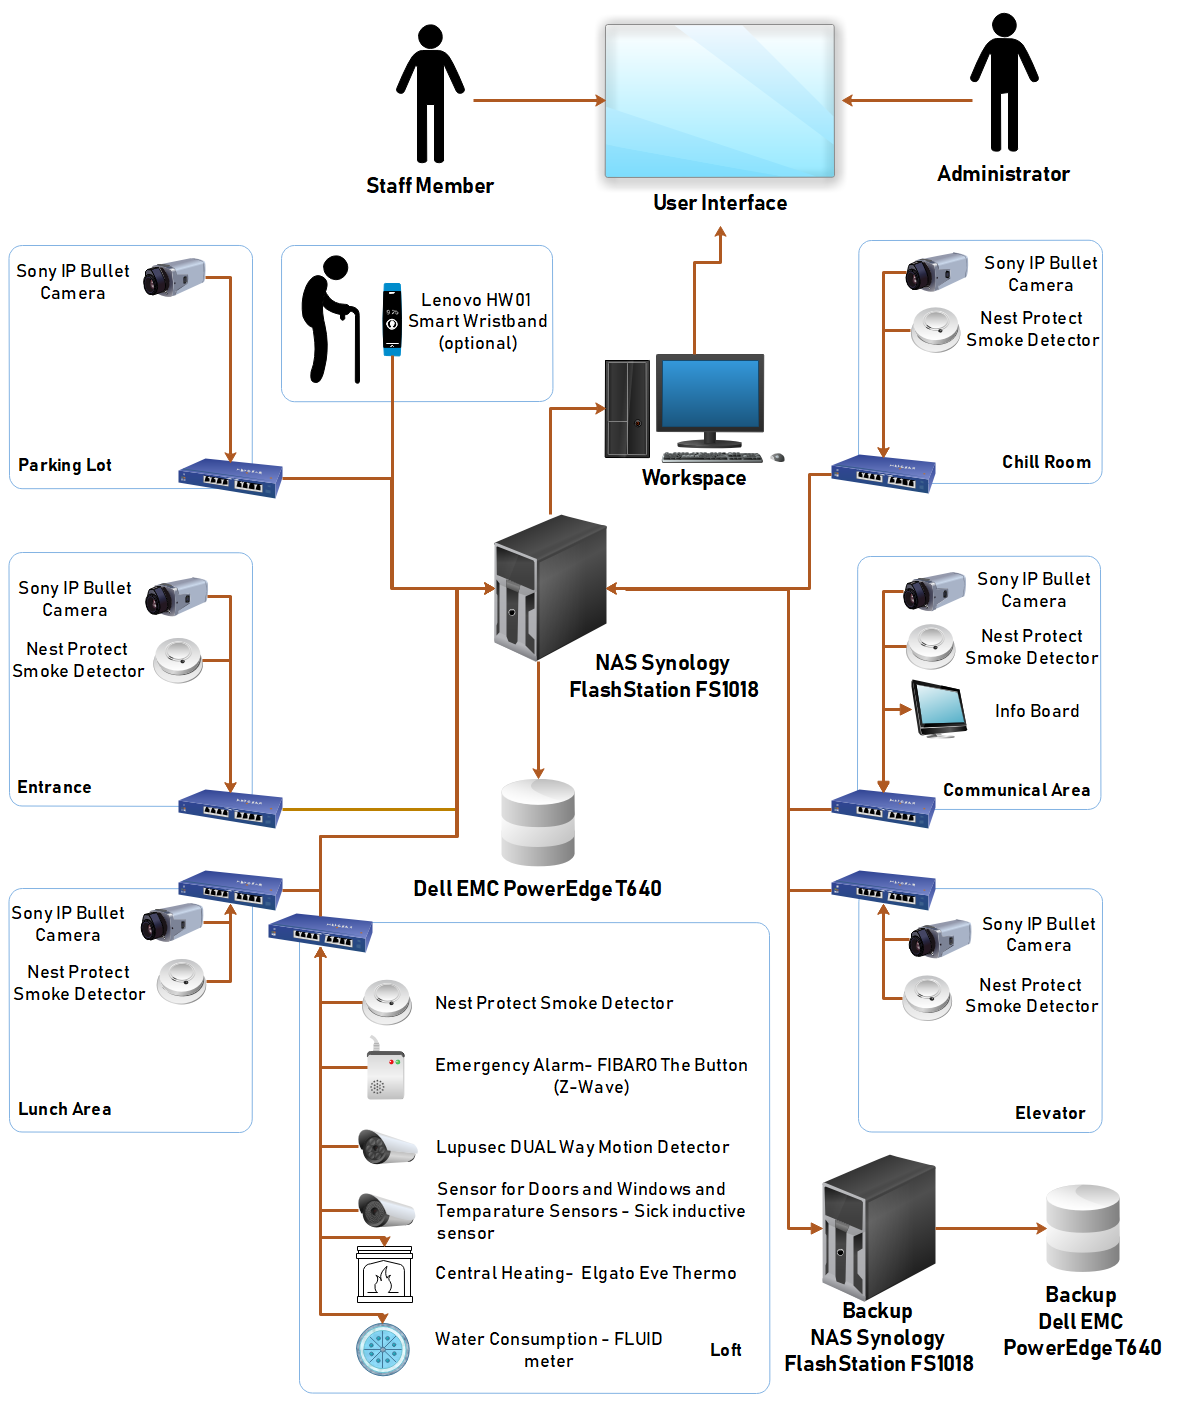
\includegraphics[width =1.0\textwidth]{images/architecture.PNG}
	\caption{Basic concept}
	\label{architecure}
\end{figure}
The figure shows the central hardware components of the iCare system and the connected devices. The rectangles represent the different rooms of the building. Each room has a HUB that communicates with the central server of the iCare system. In each room, the devices shown in the associated rectangle are installed as part of the iCare system, which communicate with the room's HUB via a wireless connection. This way, the required data reaches the server and is persisted in a database if required. The iCare server uses a RAID 2 backup system with a backup database to ensure the safety of the aquired data. The data can be accessed by employees or the administrator from any workspace using a web user-interface. The authorisation specified in the specification applies to the access to areas which show protected contents. In addition, patients can be given wristbands which monitor their vital functions on a voluntary basis or by order of a doctor. These wristbands communicate with the central server via a wireless connection and transmit the recorded data in real time.
\section{Project Plan}
\label{sec:org8452a3e}
At the beginning of a project, it is important to set up a project plan for scheduling over the entire project period and determine when certain tasks need to be completed. This simplifies the allocation of resources and can reveal problems at an early stage in the project's development. Resources can also be allocated to the individual tasks within a project plan. The number of resources available can vary within a project. It depends on how many people are involved in the project and how much time they can invest in the project. Of course, the performance of the individual team members also plays a role. The expected effort for the individual tasks is measured in hours. These are recorded for each individual task in the project plan. In addition, there is a progress bar, which is moved by the person responsible for the task during processing according to their own judgement. This allows the project manager in charge to quickly gain an overview of the progress of the individual tasks and identify where problems may occur. Planhammer\footnote{https://planhammer.io/}'s online project management tool was used to create and edit the project plan. Figure \ref{project-plan1} and figure \ref{project-plan2} shows the status of the project plan at the beginning of march.
% Ab hier im Querformat
\begin{landscape}
% Header entfernt, damit das Bild mehr Platz hat
\thispagestyle{plain}
%\newgeometry{
%  	left=3cm,
%	right=3cm,
%	top=2cm,
%	bottom=4cm,
%	bindingoffset=5mm
%}
\begin{figure}[H]
	\centering
	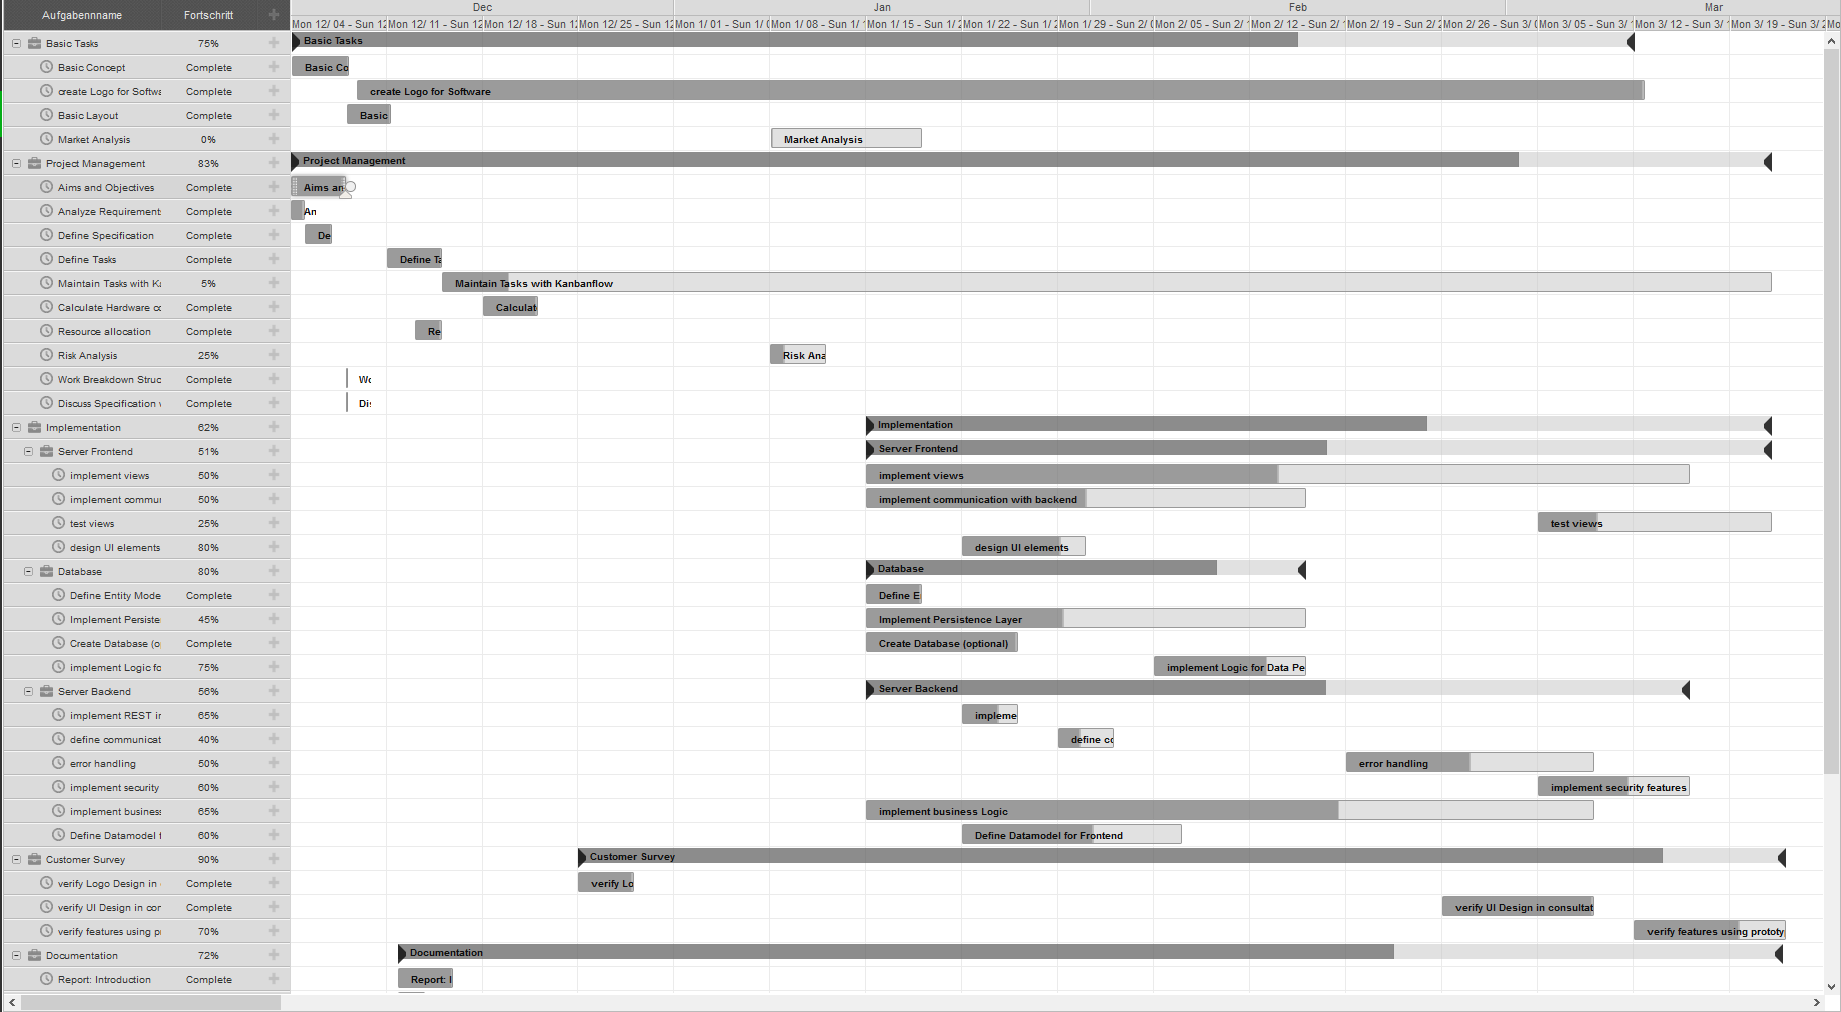
\includegraphics[width =1.4\textwidth]{images/Projectplan1.png}
	\caption{Project plan part 1}
	\label{project-plan1}
\end{figure}
\pagebreak
% Header entfernt, damit das Bild mehr Platz hat
\thispagestyle{plain}
\begin{figure}[H]
	\centering
	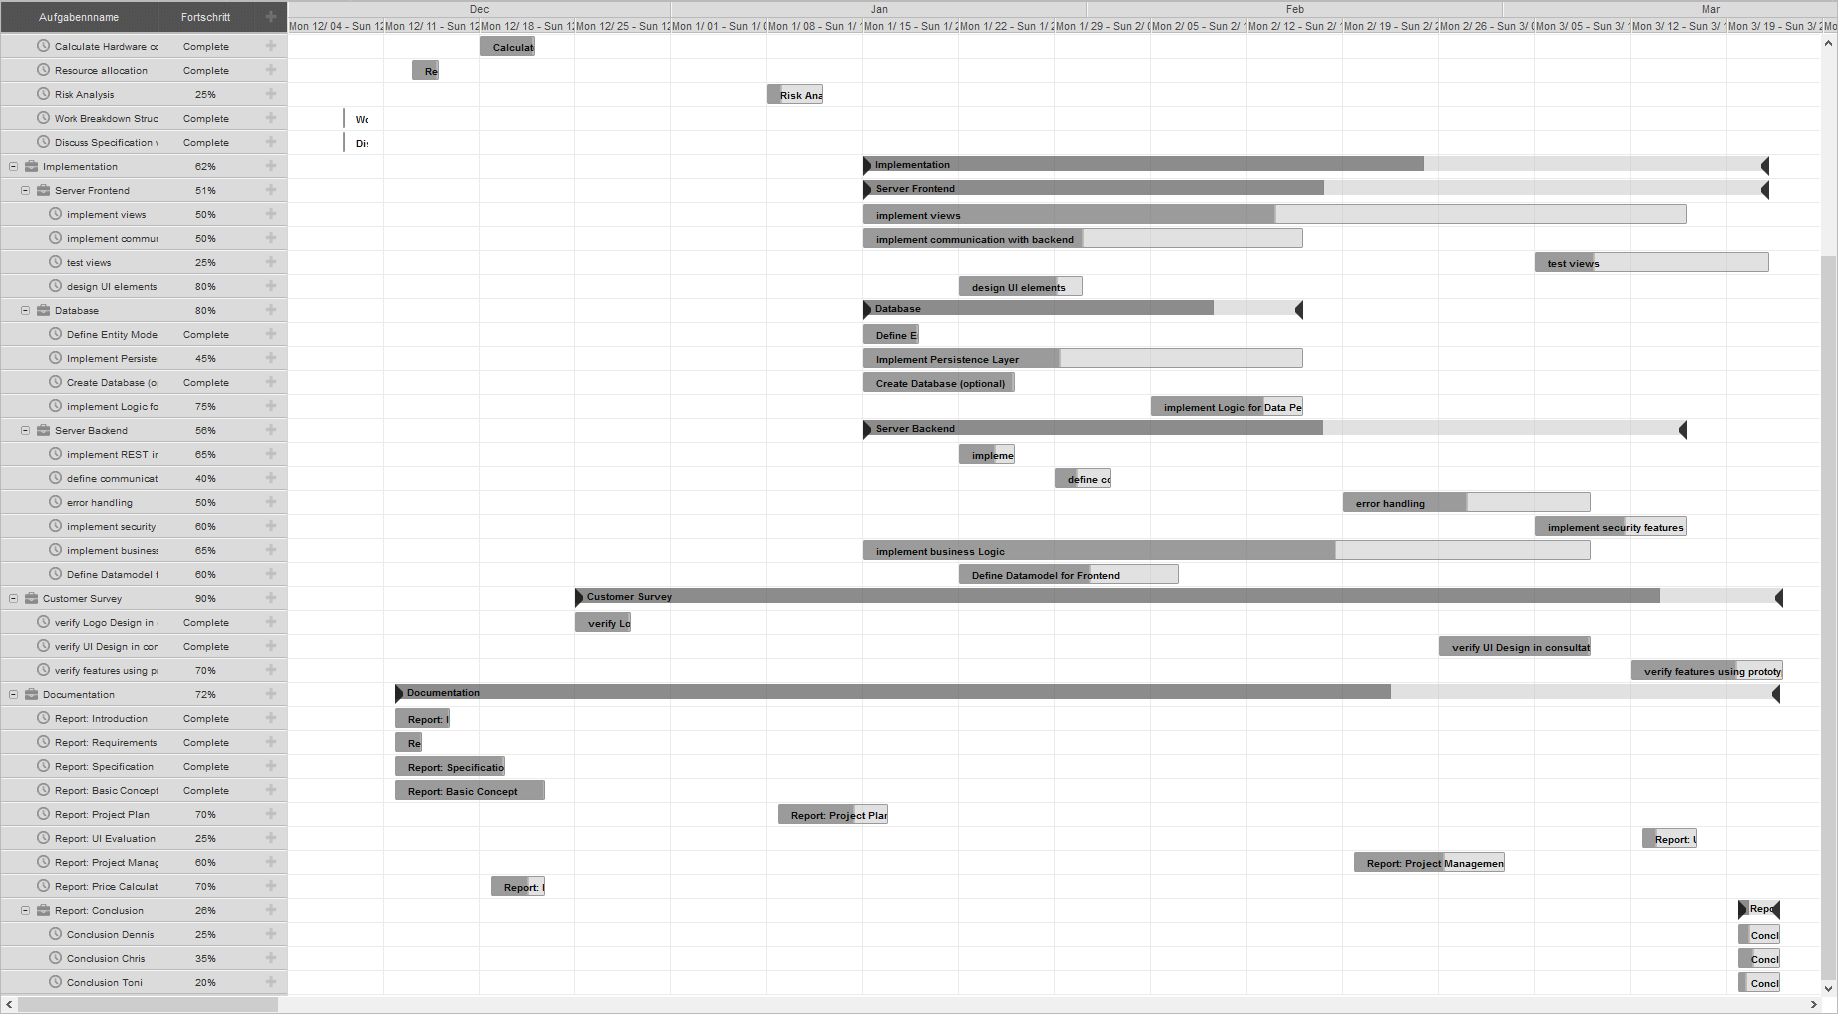
\includegraphics[width =1.4\textwidth]{images/Projectplan2.png}
	\caption{Project plan part 2}
	\label{project-plan2}
\end{figure}
%\restoregeometry
\end{landscape}
% Ab jetzt wieder hochkant
In order to get a better overview of which tasks have already been completed, which tasks are still in progress and which are still completely open, the large tasks have been split into many smaller parts. This also makes it easy to identify which periods were planned for which type of tasks. The start of the implementation on January 15th, for example, is very easy to find, as many tasks related to the implementation of the system start here. As can be seen by the progress bars, much of the implementation and documentation has already been completed. However, all activities that require an operational product such as the evaluation of user interfaces are still in progress.
\subsection{Resource Plan}
\textbf{// TODO: Tool für Resourcenplanung suchen !!!}
\section{Tracking Work}
Since the project plan is already fixed at the beginning of the project and is only used for planning, another tool is needed to keep track of the work in the course of the project. This allows the team to react to smaller, short-term changes in planning. For this purpose, the free website tool KanbanFlow\footnote{https://kanbanflow.com} was used. Kanban is a method of production process control that is often used in agile process models in software development. The various tasks from the project plan are further broken down into smaller subtasks, each of which represents a card on the virtual Kanban board. The board consists of four different sections:
\begin{itemize}
	\item To-do
	\item In Progress
	\item In Test
	\item Done
\end{itemize}
Each task can be moved freely between the sections by each project team member. However, since the tasks are handled under the responsibility of the person who created them, it is advisable that only this person moves the task. Deadlines, cost estimates and subtasks can also be defined for each task. The colour of the cards can also be set. It is advised to establish a certain pattern. In this case, the colors are assigned to the individual persons who handle the tasks. Figure \ref{kanbanflow} shows a screenshot from the online tool from March 12th.
% Ab hier im Querformat
\begin{landscape}
	% Header entfernt, damit das Bild mehr Platz hat
	\thispagestyle{plain}
	\begin{figure}[H]
		\centering
		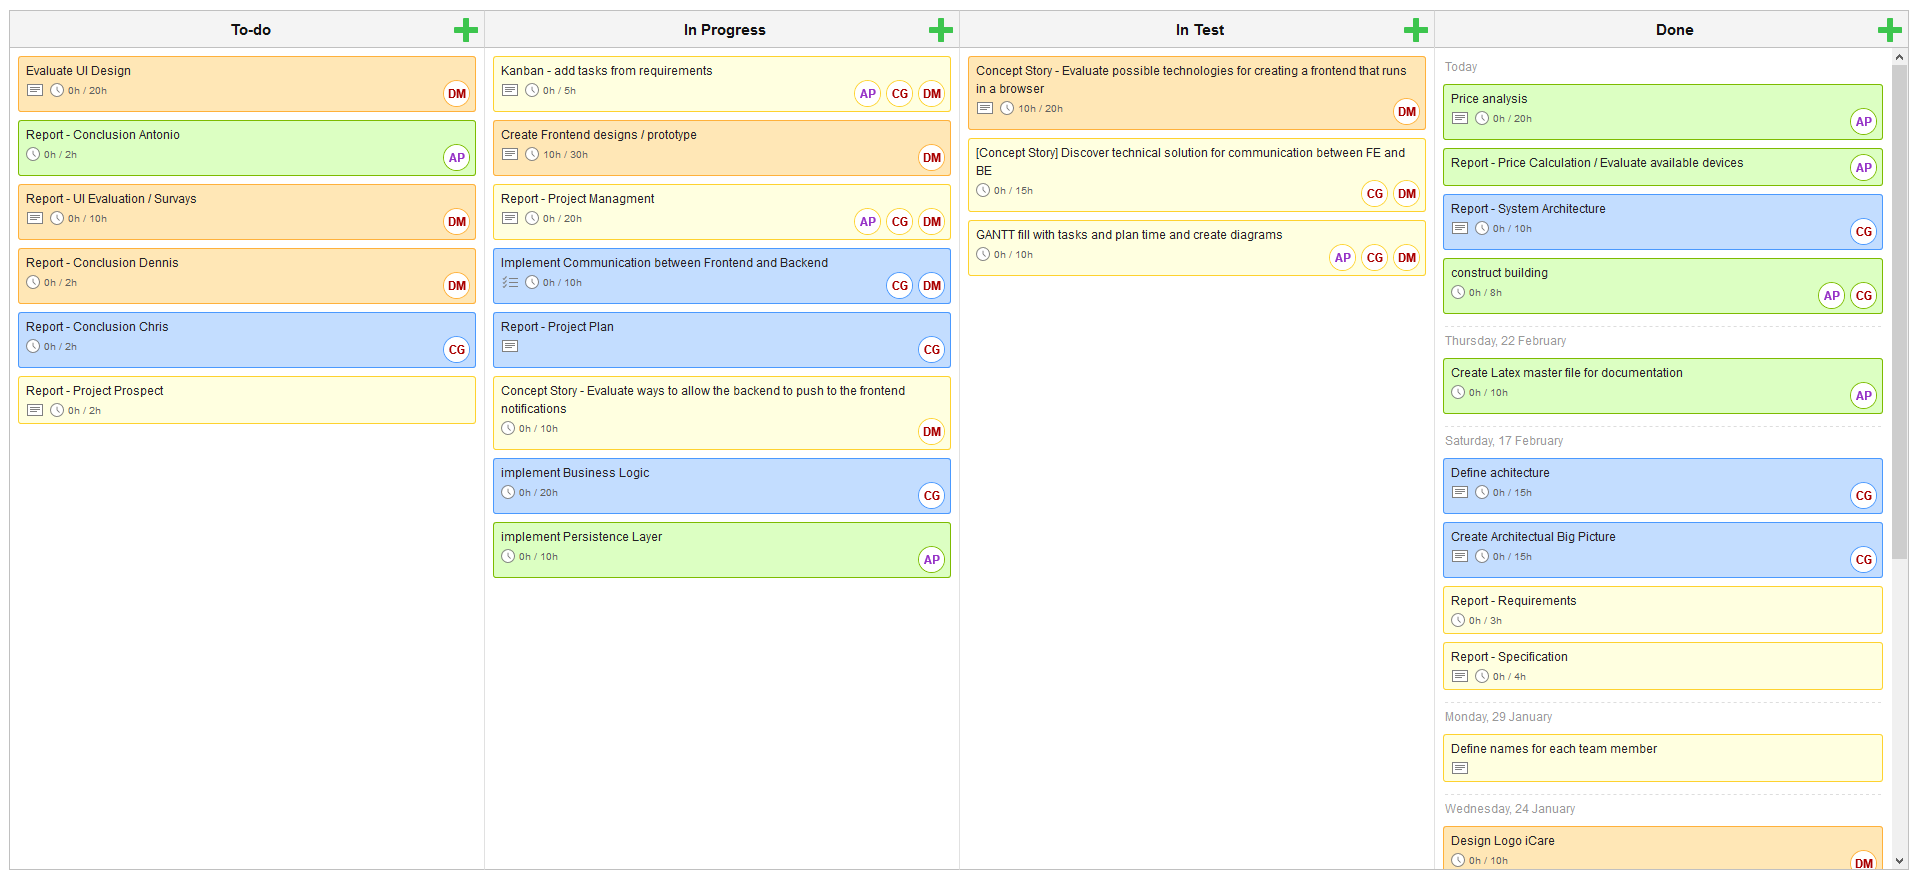
\includegraphics[width =1.4\textwidth]{images/kanbanflow.PNG}
		\caption{Maintaining task with KanbanFlow}
		\label{kanbanflow}
	\end{figure}
	%\restoregeometry
\end{landscape}
% Ab jetzt wieder hochkant
\input{"workloads"}